\documentclass[10pt,a4paper]{article}
\usepackage[utf8]{inputenc}
\usepackage{amsmath}
\usepackage{amsfonts}
\usepackage{amssymb}
\usepackage{graphicx}
\usepackage{hyperref}
\begin{document}

%Proposal follows a well-organized structure and would be readily understood by its intended audience. Each section is written in a clear, concise and specific manner. Few grammatical and spelling mistakes are present. All resources used and referenced are properly cited.

\begin{titlepage}
	\centering
	\vspace{1cm}
	{\scshape\Large Udacity 2018: Capstone Project \par}
	\vspace{1.5cm}
	{\huge\bfseries Forecasting time series with machine learning\par}
	\vspace{1.5cm}
	{\large\bfseries with applications to currency exchange rates \par}
	\vspace{2cm}
	{\Large\itshape Author: Oscar Javier Hernandez\par}
	\vfill

% Bottom of the page
	{\large \today\par}
\end{titlepage}


\section{Domain background}
%The project's domain background — the field of research where the project is derived;


%Student briefly details background information of the domain from which the project is proposed. Historical information %relevant to the project should be included. It should be clear how or why a problem in the domain can or should be solved. %Related academic research should be appropriately cited. A discussion of the student's personal motivation for %investigating a particular problem in the domain is encouraged but not required.

A set of data that is indexed by time is known as a time series. They appear in many different fields, such as statistics, physics, finance, economics, biology, or even business \cite{Adhikari_2013}. Because of their wide applicability, it is important to generate accurate forecasts of time series data. These forecasts are generated using specific mathematical models or algorithms which are trained on a subset of the past values of a given time series. For the purpose of simplifying future discussions, we will adopt the following notation for a time series, denoted $X(t)$ or $X_t$, as
\begin{equation}
\lbrace X(t); t=0,1,... \rbrace.
\end{equation}
Where $t$ denotes the time-index of the series. One of the simplest models for a time series is the ARIMA (Auto regressive integrated moving average) model. This model is denoted as ARIMA$(p,q,d)$, and assumes that the time series $X_t$ has the form
\begin{equation}
X_{t} = \mu +\epsilon_t+ \sum_{i=1}^p \phi_i L^i \left[ (1-L)^d \right] X_{t-i} + \sum_{j=1}^q \theta_j \epsilon_{t-j},
\end{equation}  
where $\lbrace \phi_i | i=1,...,p \rbrace$, $\lbrace \theta_i | i=1,...,q \rbrace$ are model parameters and $L$ is the lag operator defined as $L X_t = X_{t-1} $. The term $\epsilon_{t}$ denotes the error terms, assumed to be independent, identically distributed random variables sampled from a zero-mean, normal distribution. The value $\mu$ denotes the average of this model. ARIMA models can be applied to make forecasts of stationary time series ( defined as a time series whose mean, variance and auto correlation does not change over time), or to a time series that can be transformed into a stationary time series. However, there are other state-of-the-art machine learning methods that can be used to model time series methods. Which will the main goal of this project.
%[https://www.itl.nist.gov/div898/handbook/pmc/section4/pmc442.htm]

One important type of financial time series is the exchange rate between different currencies (Fig.~\ref{fig:EURUSD example}). An exchange rate, is the rate at which one currency will be exchanged for another. There are many factors that can influence this rate, such as balance of payments, interest rate levels, inflation levels and other economical factors which are beyond the scope of this project \cite{Patel_2014}. %[http://www.ijaiem.org/volume3issue3/IJAIEM-2014-03-05-013.pdf]

\begin{figure}[h]
\begin{center}
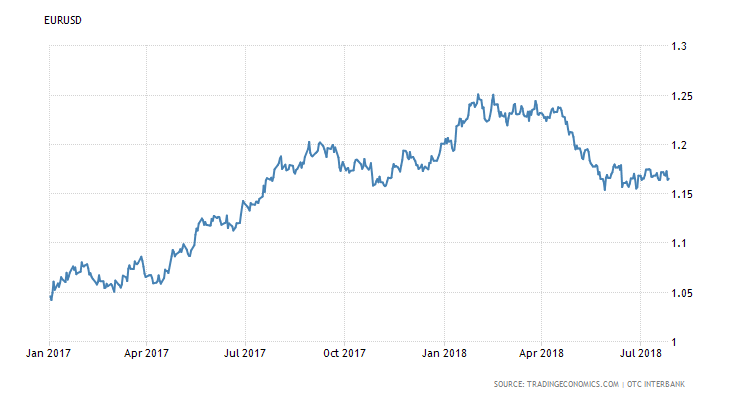
\includegraphics[scale=0.5]{EURUSD.png}
\caption{The exchange rate from EUR to USD from Jan 2017 to Jul 2018.}
\label{fig:EURUSD example}
\centering
\end{center}
\end{figure}

Because of the relevance of exchange rates to the global financial trade, it is very important to make accurate forecasts of how exchange rates will change in the future. The ultimate goal of this capstone project will be to analyze basic time series and apply machine learning methods to make forecasts about currency exchange rates.\\

% ARIMA https://arxiv.org/pdf/1508.07534.pdf

My personal motivation for working on time series is to use it to take advantage of the best exchange rates. As someone who lives abroad in a country that uses a different currency, I often need to transfer money to and from my different bank accounts. These transfers are subject to fluctuating currency exchange rates. Without a way to predict what the exchange rate will be for the time of the transfer, I end up losing money in these transfers. Therefore, I am interested in developing a way to forecast the exchange rates so that I can minimize the loses during these transfers.   



\section{Problem statement}
%A problem statement — a problem being investigated for which a solution will be defined;

% Student clearly describes the problem that is to be solved. The problem is well defined and has at least one relevant potential solution. Additionally, the problem is quantifiable, measurable, and replicable.

The main objective of this project will be to use classical and more recent machine learning techiques to make forecasts of different time series with the goal of applying the best methods to predict currency exchange rates. The simplest model that we will use is the ARIMA model, defined in the previous section as the baseline model, along with a linear regression model. The ARIMA model has been shown to be adequate in estimating the exchange rates of certain currencies Ref.~\cite{Mong_2016}. We will then use different neural networks architectures such as the feed forward and recurrent networks, as in Ref.~\cite{Chaudhuri_2016,Oancea_2014,Pant_2018}, to make predictions of time series and use our baseline models and root mean square differences to quantify and compare the performance of our different architectures.
%https://arxiv.org/pdf/1508.07534.pdf ARIMA

\section{Data sets and inputs}
%The datasets and inputs — data or inputs being used for the problem;

% The dataset(s) and/or input(s) to be used in the project are thoroughly described. Information such as how the dataset or input is (was) obtained, and the characteristics of the dataset or input, should be included. It should be clear how the dataset(s) or input(s) will be used in the project and whether their use is appropriate given the context of the problem.

In order to get a good understanding of forecasting methods we will use a number of different data sets that have more regular patterns for testing the different forecasting methods before applying the algorithm to the financial data sets. In all cases, the data sets will contain the date $t$ along with the value of the feature $X_t$. The data sets that we will use for the project are the following,

\begin{enumerate}
   \item Sunspot data
   \begin{itemize}
   \item A data set containing the number of sunspots from 1771-1869\\ \url{http://bit.ly/1yFUqWY}
   \item A data set containing the number of sunspots from 1970-1995\\ \url{http://bit.ly/1x9kgSm}
   \item This data set is well known, and will be used to test the different forecasting models.
   \end{itemize}
   \item Monthly U.S air passenger miles January 1960 through December 1977
   \begin{itemize}
   \item \url{http://bit.ly/1HHh9ry}
   \item Another well known data set having both seasonal and linear trends. It will be used for bench marking.
   \end{itemize}   
    \item Total annual rainfall in inches, for London England
   \begin{itemize}
   \item The time range is between 1813-1912
   \item \url{http://bit.ly/1gok63g}
   \end{itemize}       
   \item Mean daily temperature (Celsius), of the Fisher river near Dallas
   \begin{itemize}
   \item The date range is between Jan 01,1988 until Dec 31, 1991.
   \item \url{http://bit.ly/18f14sz}
   \item This data set will be used for testing the algorithms.
   \end{itemize}
      \item The Kaggle EURUSD Data set
   \begin{itemize}
     \item The data contains Forex EURUSD currency rates in 15-minute slices (OHLC - Open High Low Close, and Volume).  BID price only.
     \item The data ranges from Jan 1, 2010 until Jan 1, 2017.\\
     \url{https://www.kaggle.com/meehau/EURUSD/home}
   \end{itemize}
   
         \item Historical EURCAD data set
   \begin{itemize}
     \item The data contains historical data, BID price only.
     \item The data ranges from Oct. 24, 2004 until July 21, 2018.
     \item The data was downloaded online from\\ \url{https://www.dukascopy.com/swiss/english/marketwatch/historical/}
   \end{itemize}   
   
   \item Exchange rate of the Australian dollar 
   \begin{itemize}
   \item The date range is from 1969-1995
   \item \url{http://bit.ly/1x9kgSm}
   \end{itemize}
\end{enumerate}


\section{Solution statement}
%A solution statement — a the solution proposed for the problem given;

% Student clearly describes a solution to the problem. The solution is applicable to the project domain and appropriate for the dataset(s) or input(s) given. Additionally, the solution is quantifiable, measurable, and replicable.


The solutions that we purpose for this project is to use a feed forward artificial neural networks \cite{Chaudhuri_2016}, along with a recurrent network \cite{Pant_2018} to make time series predictions. If time is available, we also propose to use a generative adverserial network (GAN) which has shown some promise for time series models in the medical field \cite{Esteban_2017}. We will train these neural network architectures using the data sets described in the previous sections and make predictions. We will use the evaluation metrics described in later sections to compare the performance of these solutions against the benchmark models in the next section.



\section{Benchmark model}
%A benchmark model — some simple or historical model or result to compare the defined solution to;

% A benchmark model is provided that relates to the domain, problem statement, and intended solution. Ideally, the student's benchmark model provides context for existing methods or known information in the domain and problem given, which can then be objectively compared to the student's solution. The benchmark model is clearly defined and measurable.

For the benchmark models, we will use two well known models, a simple linear regression model and an ARIMA model. The linear regression model will assume the following simple short term relation between points in the time series,
\begin{equation}
X_{t} = a\cdot t + b.
\end{equation}
The parameters to be fit are slope, $a$, and the intercept, $b$. The {\bf sklearn} package in python can be used to fit lines to the data.\\

The second model that we will use to benchmark our machine learning algorithms will be the ARIMA$(p,q,d)$ model defined in the introduction. The {\bf stats} package in python contains numerical routines that will fit an ARIMA model to a time series \cite{Vincent_2018}.\\

Both the linear and the ARIMA model will be our basic models that will be used to compare the performance of our neural network based machine learning models using the evaluation metrics in the next section. This will allow us to determine if the neural network machine learning methods are in fact better than the base models.


\section{Evaluation metrics}
%A set of evaluation metrics — functional representations for how the solution can be measured;

% Student proposes at least one evaluation metric that can be used to quantify the performance of both the benchmark model and the solution model presented. The evaluation metric(s) proposed are appropriate given the context of the data, the problem statement, and the intended solution.

There are several metrics that we can use to evaluate the predictions of our models Ref.~\cite{Adhikari_2013}, however, for our project we will focus on three commonly used metrics. We will first define some terminology, the forecast error, $e_t$, is given by
\begin{equation}
e_{t} = X_t - F_t,
\end{equation}
where $X_t$ is the value of the time series at time step $t$, and $F_t$ is the forecasted value at the same time step. The three metrics that we will use for our project are
\begin{enumerate}
\item  The Mean Absolute Percentage Error (MAPE)
\begin{itemize}
\item $\text{MAPE} = \frac{1}{N}\sum\limits_{t=1}^{N} \left| \frac{e_{t}}{X_t} \right| \cdot 100 $
\end{itemize}

\item  The Mean square error (MSE)
\begin{itemize}
\item $\text{MSE} = \frac{1}{N}\sum\limits_{t=1}^{N} e^2_{t} $
\end{itemize}

\item  The Mean absolute error (MAE)
\begin{itemize}
\item $\text{MAE} = \frac{1}{N}\sum\limits_{t=1}^{N} |e_{t}| $
\end{itemize}

\end{enumerate}
\noindent
In these three cases, the smaller the value of the MAPE, MSE, and MAE, then the better the model.



\section{Project design}
%An outline of the project design — how the solution will be developed and results obtained.

%Student summarizes a theoretical workflow for approaching a solution given the problem. Discussion is made as to what strategies may be employed, what analysis of the data might be required, or which algorithms will be considered. The workflow and discussion provided align with the qualities of the project. Small visualizations, pseudocode, or diagrams are encouraged but not required.

The project design will consist of the following steps

\begin{enumerate}
\item Data preprocessing
\begin{itemize}
\item First we can perform transformations on the data to remove seasonal patterns, linear trends for each of the data sets that we will consider.
\item We can also perform different smoothing operators, like the running average, or exponential smoothing.
\end{itemize}

\item Splitting the data
\begin{itemize}
\item We will split the data into testing and training.
\item The amount will be (80$\%$) training and (20$\%$) testing, but we will evaluate the models using different amounts of training data.
\end{itemize}

\item Training
\begin{itemize}
\item The models that we will train are: Linear regression, ARIMA, and at least two different neural network architectures described in the previous sections.
\item Once the data has been split into training and testing, then we will use the training data set to determine the model fit parameters, and make predictions on the testing set.
\item The model parameters will be varied during this phase, until the objective function is minimized. The objective function will be either the MAPE, MSE or MAE metric.
\item For each of the trained models, we will compare the value of the metrics defined in the previous section.
\end{itemize}



\item Forecasts
\begin{itemize}
\item Once the training phase is complete, then the model will be used to make predictions of the future.
\item We will also attempt to quantify the uncertainty associated with the forecasts of the various models. 
\end{itemize}


\end{enumerate}


\begin{thebibliography}{9}

\bibitem{Adhikari_2013}
R. Adhikari and R. K. Agrawal, An Introductory Study on Time Series Modeling and Forecasting, 2013, [arXiv:1302.6613] \url{https://arxiv.org/abs/1302.6613}.

\bibitem{Mong_2016}
Research Journal of Finance and Accounting www.iiste.org
ISSN 2222-1697 (Paper) ISSN 2222-2847 (Online)
Vol.7, No.12, 2016 \url{http://iiste.org/Journals/index.php/RJFA/article/viewFile/31511/32351}.

\bibitem{Patel_2014} P. J. Patel,  N. J. Patel and A. R. Patel, IJAIEM 3, 3, 2014. \url{http://www.ijaiem.org/volume3issue3/IJAIEM-2014-03-05-013.pdf}

\bibitem{Oancea_2014} B. Oancea, S. Cristian Ciucu, Proceedings of the CKS 2013, [arXiv:1401.1333] \url{https://arxiv.org/abs/1401.1333}.

\bibitem{Chaudhuri_2016} T. D. Chaudhuri and I. Ghosh,	Journal of Insurance and Financial Management, Vol. 1, Issue 5, PP. 92-123, 2016,  [arXiv:1607.02093] \url{https://arxiv.org/abs/1607.02093}.

\bibitem{Pant_2018} Pant, N. (2017, September 07). A Guide For Time Series Prediction Using Recurrent Neural Networks (LSTMs). Retrieved from \url{https://blog.statsbot.co/time-series-prediction-using-recurrent-neural-networks-lstms-807fa6ca7f}.


\bibitem{Vincent_2018} Vincent, T. (2018). ARIMA Time Series Data Forecasting and Visualization in Python | DigitalOcean. [online] digitalocean.com. Available at: \url{https://www.digitalocean.com/community/tutorials/a-guide-to-time-series-forecasting-with-arima-in-python-3} [Accessed 29 Jul. 2018].

\bibitem{Esteban_2017} C. Esteban, S. L. Hyland and G R\"{a}tsch, \url{https://github.com/ratschlab/RGAN} [arXiv:1706.02633]. 

\end{thebibliography}
\end{document}